\chapter{Proposed model}
\label{chap:Proposedmodel}

\section{Framework overview}
\label{sec:framework}

The proposed model is a full flow from data stream generation, anomaly detection with autoencoder-based model and online model incremental updating. \Fref{fig:flowchart} shows the general pipeline. The first received batches of streaming data are used for decision of model hyperparameters and the model initialization. Hyperparameters includes the hidden layer size, batch size, input window length as well as the number of epochs. Once the hyperparameters are learned, an autoencoder will be constructed and initialized with random weights. A subset of the streaming data is used for initial model training (only normal data used for training). Furthermore, the model is used for online anomaly detection, and evaluated based on the label provided by experts if available, or otherwise the model trust its prediction, and collect hard examples for retraining. Model will be retrained when the retraining condition is triggered. As shown in Algorithm \ref{alg:pipeline}, if a batch of streaming data is available, the model will start do prediction, evaluation, and check whether current window is useful to store for later retraining. If so, the window of data will be appended to the retrain buffer, with the instance order not been destroryed. As a consequence of anomalies' rare appearance, we keep all seen anomalous windows for determination of anomaly score threshold during retraining. 


\begin{figure}[h]
\centering
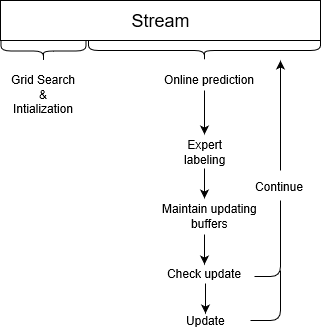
\includegraphics[width=10cm, height=10cm]{flowchart}
\caption[Online anomaly detection system flowchart]{Online anomaly detection system flowchart}
\label{fig:flowchart}
\end{figure}

\begin{algorithm}[h]
\SetKwInOut{Input}{input}
\Input{normal buffer size: SN, abnormal buffer size: SA,performance threshold: P}

\BlankLine 
needRetraining = False\;
normalBuffer = [ ]\;
abnormalBuffer = [ ]\;
\BlankLine 
 \While{True}{
%	\eIf{len(retrainBuffer) == retrainDataSize}{retrain(retrainBuffer)\;}
	 \eIf{len(normalBuffer) >= SN $\textbf{and}$ len(abnormalBuffer) >= SA}{retrain(normalBuffer, abnormalBuffer)\;}
	{
	data, labels = getBatchData()\;
   	pred = predict(data)\;
	result = evaluation(pred,labels)\;
	\ForEach {window $\textbf{in}$ data}{
	\If{$'$anomaly$ '$ $\textbf{in}$ label[window$.$index]}{abnormalBuffer$.$append(window)}
	\eIf{result[window$.$index] $>=$ P}{continue\;}{\eIf{label == $'$normal$ '$}{normalBuffer$.$append(window)\;}{continue\;}}
	
	}

	}
	}

 \caption{OnlineAnomalyDetection}
\label{alg:pipeline}
\end{algorithm}



\section{LSTMs-Autoencoder}
\label{sec:initialization}

\subsection{Encoder-decoder architecture}
\label{sec:Encoder-decoder architecture}

The LSTMs-Autoencoder is consist of two LSTM units, one as encoder and the other one as decoder. The encoder inputs are fix length vectors with shape <MB, T, D>, where MB is the number of data windows contained in a mini-batch, T is the numbers of data points within each data window, and D represents the number of data dimensionality. Here, MB and T are learned as hyperparameter in the initialization phase. And on the decoder side, it will output exactly the same format data vector for each mini-batch. The LSTM unit copies its cell state for itself as one of the cell input at next timestamp. At the last timestamp of encoder, the cell state of LSTM unit is the hidden representation of the input data vector and copied to the decoder unit as initial cell state, so the hidden information can be passed to the decoder. The size of hidden layer representation vector, namely the size of cell state is another hyperparameter need to be learn in the initialization phase. The larger the hidden vector, the more information can be captured during the process, so it is a feature highly depends on the data. Similar to previous study \cite{seq2seq}, we also train the encoder and decoder with time series in reverse order. For example, if the input data fragment are data points from timestamp t1 to t2, then the decoder will predict data point at t2 at first, and then back to t1 step by step, while this trick makes the gradient escarpment between last state of encoder and first state of decoder smaller and easier to learn. \\

In order to let the whole process happen online, the model initialization also utilizes streaming data. Once a small subset of streaming data is available, hyperparameters are learned, and then another dataset that consists only of normal data is collected from stream used for training. Assume that once an anomaly detection task is determined, the anomalous state is explicit defined and a subset of anomalous data is available for model initialization. We split the normal data into four subsets, $N_1$ for hyperparameters tuning, $N_2$ for model training, $N_3$ for early stopping, and scoring parameters learning, $N_4$ for testing. And abnormal data are split into two subsets, $A_1$ for decision of anomaly score threshold, $A_2$ for testing.

\subsection{Online anomaly detection}
\label{anomalydetection}
The autoencoder reconstructs the input with its knowledge of normal data, so if the input data contains anomalies, the reconstruction error will be obviously large due to the lack of anomalous knowledge. For input $X^{(i)}$, the reconstruction error is 

\begin{equation} \label{eq:error}
e^{(i)}=\left| X^{(i)} - X^{'(i)} \right|
\end{equation}

similar to \cite{encdecad}, the reconstruction error of data points $N_3$ is used to estimate the parameters $\mu$ and $\Sigma$of a normal distribution $\mathcal{N}(\mu,\,\Sigma)$ using maximum likelihood estimation. The anomaly score for a point $x_t^{(i)}$ is defined as 

\begin{equation} \label{eq:score}
a^{(i)}={(e^{(i)}-\mu)}^{T}{\Sigma}^{-1}{(e^{(i)}-\mu)}
\end{equation}

During the initialization phase, a anomaly score threshold $\tau$ is also learned using $N_3$ and $A_1$ as

\begin{equation} \label{eq:threshold}
\tau = argmax AUC(a(N_3),a(A_1))
\end{equation}

The anomaly score of every instance in a window is compared with the threshold, and values over the threshold are predicted as anomalies. If a window contains more than $\tau_N$ anomalous values, this window is predicted as anomaly.




\section{Online learning}
\label{sec:Onlinelearning}
However, if we consider using the model for streaming data, the autoencoder might get outdated because of the relative small and simple initialization dataset and concept drift happed along with time. So the update of model is necessary. In this section, we introduce the incremental learning function of the LSTMs-Autoencoder.

\subsection{Retraining dataset}
\label{data}

Normally when the LSTMs-Autoencoder is initialized, it is ready for online prediction. There is a multi-thread setting in the online learning architecture. A sub thread collects data instances continuously from the Kafka publisher, and in the meantime, the main thread is working on real-time anomaly detection as long as mini-batches of data is provided by the sub thread. For each single window in the mini-batch, every instance is reconstructed and calculated the anomaly score using \Fref{eq:score}. The system maintains two data buffers for retraining (\Fref{fig:buffer}), one for normal data, and the other one for anomalies.Considering the fact that a well mastered window leads to lower reconstruction error, and higher error indicates new features in the data, and we can measure this reconstruction error level by the predefined normal distribution on reconstruction error. Normal data windows with too much high score instances are regarded as not good mastered and will be appended into the normal buffer for retraining. As anomalies appear rarely in the stream, we collect all anomalous windows in the abnormal buffer for threshold determination during retraining. To this end, when a retraining process is triggered, only not well mastered normal data are used for retraining.

\begin{figure}[h]
\centering
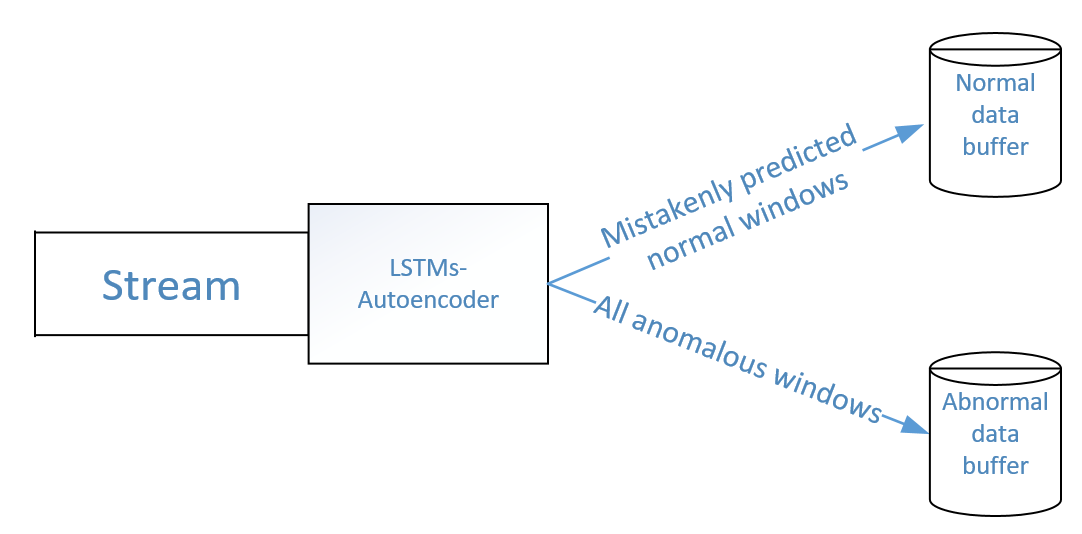
\includegraphics[width=10cm, height=5cm]{buffer}
\caption[Retraining data buffer]{Retraining data buffer}
\label{fig:buffer}
\end{figure}


\subsection{Retraining trigger}
\label{trigger}

During the online processing, if the system detected that the model doesn’t fit the current data any more, then the retraining is triggered and done with the latest collected data in the two buffers. During experiments we found that, anomalies only appears rarely in the stream, so it often happens that the model need retraining to fit the latest data, but still lack of anomaly data in the buffer to update the threshold. To this end, we separate the updating of model and threshold, namely, when the retraining is triggered, update threshold only if there is enough abnormal data, otherwise only retrain model with the normal buffer. In case of the normal buffer reaches a predefined size, the model is retrained in a sub thread while the main thread keeps processing the stream. 

\subsection{Model retraining}
\label{retraining}

Once retraining process is triggered, the model will be retrained using data from retrain buffers. Windows of normal buffer are divided into retraining set and retraining validation set. The retraining is a continuation of the initialization or previous retraining with identical data format. Parameters mu, sigma as well as threshold are learned from the retraining validation set and anomaly buffer data. The parameters are learned in the same way as in initialization phase.

\begin{algorithm}[h]
\SetKwInOut{Input}{input}
\Input{normal buffer: nBuf, abnormal buffer: aBuf}

\BlankLine 
retrainSet, valSetN = split(nBuf)\;
valSetA = aBuf\;

ModelReTrain(retrainSet)\;
mu, sigma, threshold = getParameters(valSetN, valSetA)

\caption{retrain}
\label{alg:retrain}
\end{algorithm}




